\section{Overview}
\label{sec:overview}


\begin{figure}[!tb]
  \begin{center}
    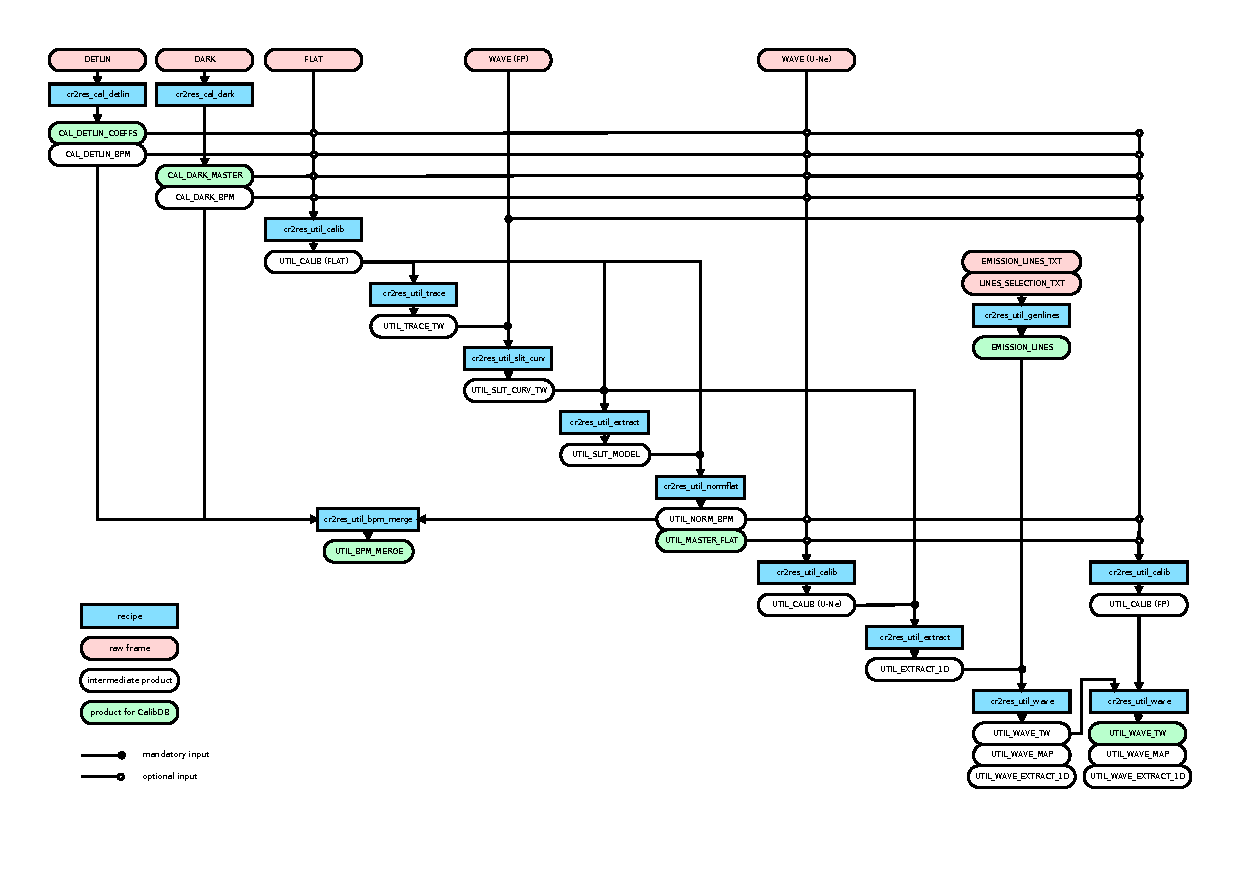
\psfig{file=figures/calib_detailed.pdf,width=0.99\linewidth}
  \end{center}
  \caption{
    \label{fig:calibflow_detailed}
    .}
\end{figure}

\begin{figure}[!tb]
  \begin{center}
    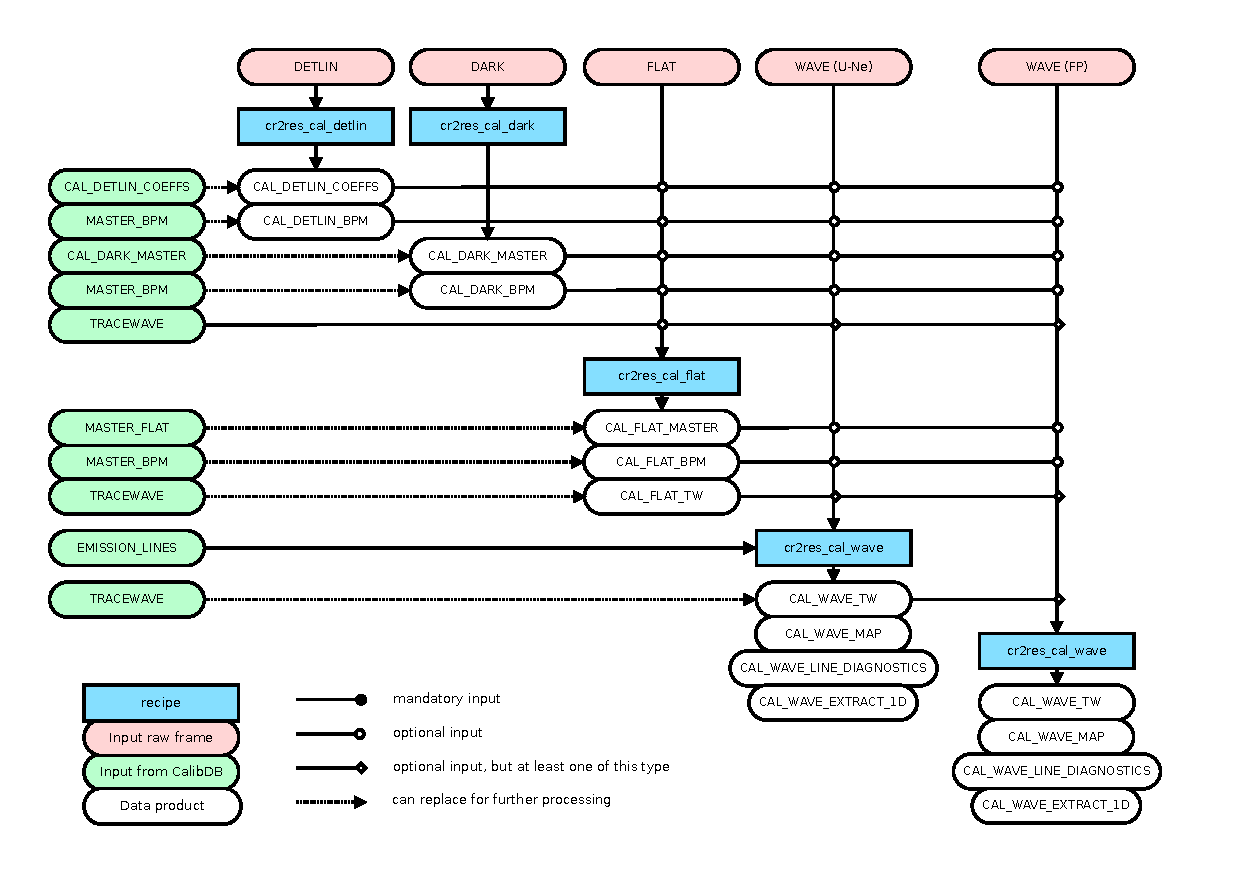
\psfig{file=figures/calib_simple.pdf,width=0.99\linewidth}
  \end{center}
  \caption{
    \label{fig:calibflow_simple}
    .}
\end{figure}



The calibrations that are needed to characterize the instrument are
\begin{enumerate}
    \item Detector linearity, "Detlin"
    \item Dark
    \item Bad Pixel Map, BPM
    \item Find order locations, "tracing".
    \item Slit tilt characterization
    \item Flat-fielding
    \item Wavelength calibration
\end{enumerate} 

The results of steps 1,2,3 and 6 are stored as separate master calibrations, respectively. Information about the orders 4,5,7 are stored together in a TW-table, as described in more detail %TODO ref.

To fully reduce a science frame, the following steps are carried out:
\begin{enumerate}
    \item Combine frames
    \item Apply master calibrations: Detlin, Dark, BPM and Flat-field
    \item Extraction of spectra, using the TW-table.
    \item (Splicing together spectra from different detectors and orders)
\end{enumerate}

